\chapter{Tecnologías}
\label{cap:introduccion}

%\chapterquote{}{}

\begin{resumen}
	En este capítulo se enumerarán las tecnologías utilizadas y su utilidad en el proyecto.
\end{resumen}

\label{cap1:sec:Motivacion}


\section{Introducción}
Para llevar a cabo el proyecto, fue necesario investigar sobre tecnologías existentes que faciliten el desarrollo del mismo [COMPLETAR]
\section{API Arasaac}
ARASAAC facilita la obtención de recursos pictográficos mediante su API\footnote{\url{https://arasaac.org/developers/api}}. Dicha API está exclusivamente disponible para aplicaciones no comerciales, tal y como indica su licencia Creative Commons.
Mediante los métodos de la API , podemos obtener materiales y pictogramas. Los materiales  son actividades, calendarios o agendas hechas con pictogramas. Respecto a los pictogramas, los métodos que hemos utilizado son.
\begin{itemize}
	\item \textbf{BestSearch}: A partir de una palabra dada retorna el identificador y otros datos como el significado o la categoría del pictograma que más se asemeje al término buscado. Además, permite buscar palabras en multitud de idiomas.
	
	\item \textbf{searchText}: Igual que \textit{BestSearch}, diferenciándose en que retorna todos los pictogramas en vez de uno solo.
	
	\item \textbf{idPictogram}: A partir del identificador obtenido anteriormente, retorna la dirección de la imagen del pictograma asociado al identificador. 
	

	
		
\end{itemize}

La API de ARASAAC está pensada para ser utilizada por múltiples aplicaciones en distintos idiomas por lo que ofrece la posibilidad, tanto en los métodos de búsqueda como los pictogramas en sí, de seleccionar qué idioma queremos usar por defecto.
Otro característica a destacar, es que todos aquellos métodos en los que se retornen pictogramas podrán ser modificados desde la propia llamada a la API. Podremos modificar desde el color de fondo, rasgos físicos o tiempos verbales entre otras muchas opciones. Podemos ver un ejemplo de ello en la Figura  \ref{fig:colorespicto} que muestra la edición del pictograma "Niño" dentro de la web de ARASAAC \footnote{\url{https://arasaac.org/pictograms/es/7176/niño}}

	% TODO: \usepackage{graphicx} required
\begin{figure}
	\centering
	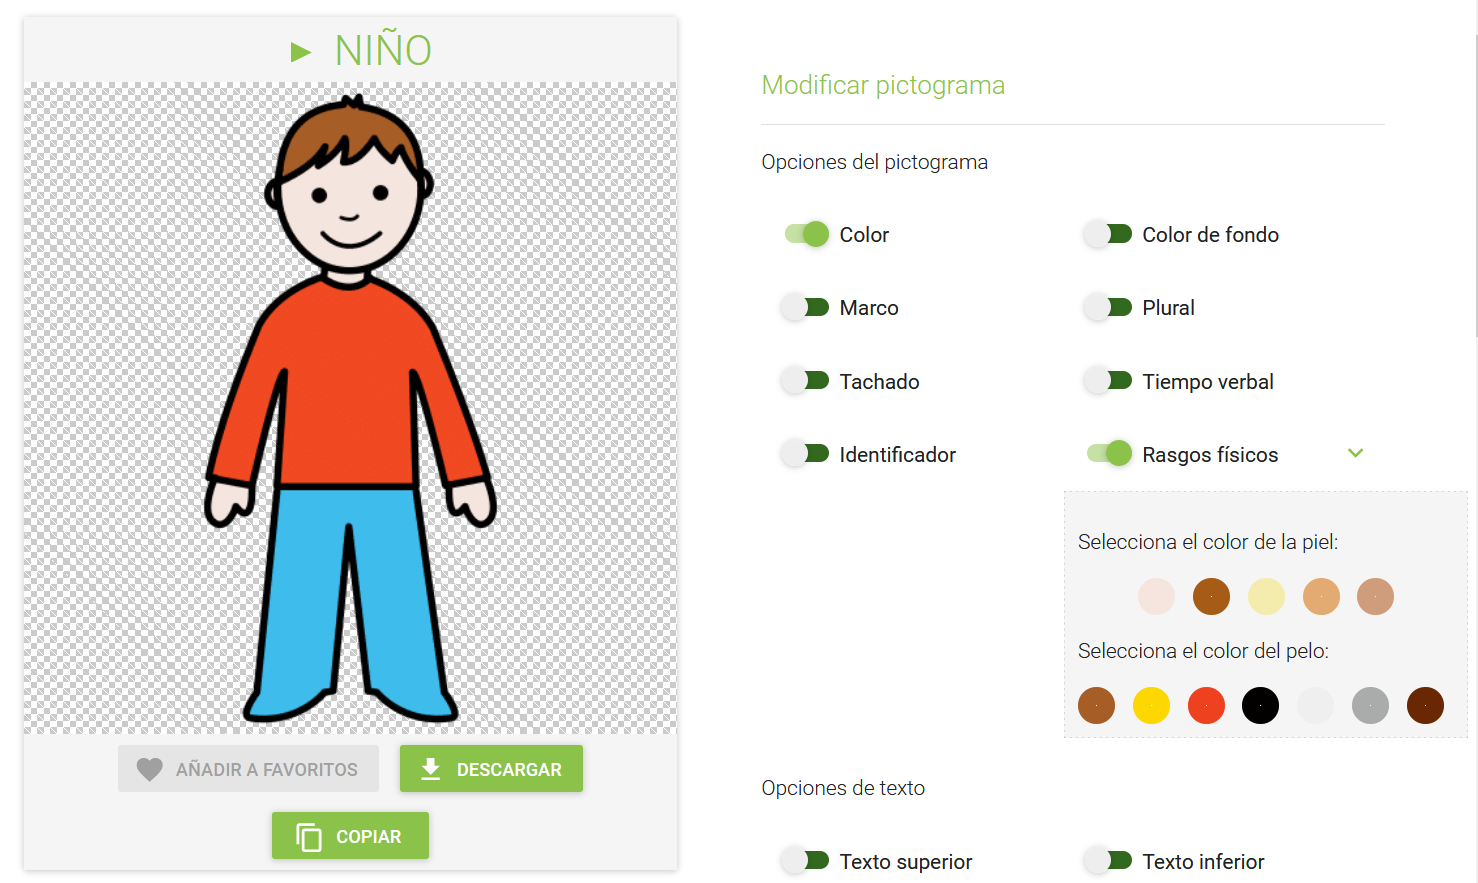
\includegraphics[width=0.7\linewidth]{Imagenes/Bitmap/coloresPicto}
	\caption{Ejemplo de cómo se puede modificar el color de pelo y tono de piel de un pictograma entre otras opciones, en la web de ARASAAC}
	\label{fig:colorespicto}
\end{figure}

\section{React}

React es una librería de Javascript pensada para desarrollar interfaces de usuario. Esta librería fue desarrollada por Facebook buscando la creación de interfaces de una manera sencilla y con un alto rendimiento. 
React permite desarrollar tanto aplicaciones web como aplicaciones móviles de una manera ordenada y con menos líneas de código respecto a otros lenguajes como Javascript puro. El hecho de que React permita estructurar los distintos componentes de una aplicación ayuda tanto al desarrollo como mantenimiento de esta.
Otra característica importante de React es que ya tiene implementado muchas funcionalidades por lo que puede ayudar a reducir el tiempo de desarrollo de la aplicación, un ejemplo de esto es el hecho de tener las vistas asociadas a los datos. Esto permite que los datos mostrados se actualicen automáticamente sin necesidad de escribir nuevos fragmentos de código.

Respecto a otros Frameworks como Angular, vemos que React no ofrece todas las funcionalidades de un framework completo. Esto no supone ningún impedimento para desarrollar la aplicación con React pero habrá que adaptar nuestro código al ecosistema que ofrece.

\section{Drag and Drop}

React Drag and Drop\footnote{\url{https://react-dnd.github.io/react-dnd/about}} Es una biblioteca que permite arrastrar componentes en React. Su principal uso en la aplicación, es la recolocación de los componentes del tablero de manera cuadriculada. Esto permite colocar con precisión los elementos en el tablero, lo cual era un requisito indispensable para poder hacer tableros organizados. De otra manera podrían quedar algunos componentes unos pocos píxeles por encima de otro, dando un resultado poco profesional.

\section{JSZip}

JSZip \footnote{\url{https://stuk.github.io/jszip/}} es una biblioteca de javascript que mediante una API permite crear y cargar archivos comprimidos en formato \textit{ZIP}. Será el método para importar y exportar proyectos a la aplicación.
\begin{itemize}
	\item \textbf{Generar ZIP}: Crea un zip con todo lo que haya creado el usuario, como las fotos que haya subido, la posición de los pictogramas colocados y su información asociada (Por ejemplo, si se ha cambiado la descripción de un pictograma)
	\item \textbf{Cargar ZIP}: Al subir un ZIP, vuelve al estado cuando fue generado.
\end{itemize}	


\textcolor{red}{CAMBIAR}


\section{Prototipos Tecnológicos}

Durante las primeras etapas del desarrollo, creamos algunos prototipos para familiarizarnos con las tecnologías imprescindibles para crear la aplicación. Estas fueron el acceso a la API de ARASAAC \footnote{\url{https://arasaac.org/developers/api}} y desplazar elementos en una aplicación web.

\subsection{API ARASAAC}

Para probar el acceso a la API se creó un buscador de pictogramas independiente para comprender el funcionamiento de la API y las posibilidades que ésta ofrece. Aunque inicialmente simplemente muestra el pictograma de una palabra introducida. Pero más adelante en el desarrollo, explotamos la posibilidad de cambiar el color de pelo y tono de piel de los pictogramas que lo permiten.


\subsection{React Drag and Drop:}

Otro objetivo es el de la interacción de los componentes en una superficie cuadriculada. Tras experimentar con distintas bibliotecas de JavaScript como Interact JS \footnote{\url{https://interactjs.io/}} no obtuvimos el resultado esperado pues el desplazamiento de los objetos no era lo suficientemente preciso.

React tenía la biblioteca Drag and Drop que permite desplazar los componentes. La principal diferencia entre Drag and Drop y Interact JS, es que al mover un elemento, “Interact JS”  deja unos píxeles de diferencia y “Drag and Drop.” permite mover objetos en intervalos definidos, como poder mover un objeto de 10 píxeles en 10 píxeles.